\documentclass{beamer}

\beamertemplatenavigationsymbolsempty
\usetheme{Warsaw}

\title{Computer Graphics -- Homework 3}
\author{Tran Phong Binh}
\institute{Student ID: 110062421}
\date{\today}

\begin{document}

\begin{frame}
  \titlepage
\end{frame}

\begin{frame}
  \frametitle{Executable}
  \begin{itemize}
    \item The shaders must be in the same folder as the binary's in order to execute the program.
  \end{itemize}
  \begin{figure}
    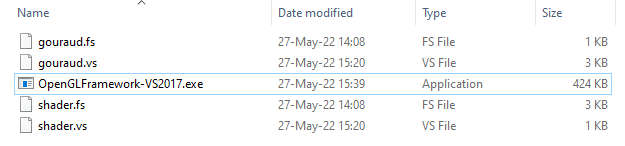
\includegraphics[width=\textwidth]{executable}
    \caption{Executable folder}
  \end{figure}
\end{frame}

\begin{frame}
  \frametitle{Static Key Controls}
  \begin{itemize}
    \item G: nearest/linear magnification
    \item B: nearest-mipmap-linear/linear-mipmap-linear minification
    \item $\rightarrow$: next eye texture
    \item $\leftarrow$: previous eye texture
  \end{itemize}
\end{frame}

\begin{frame}
  \frametitle{Texture Wrapping}
  \begin{itemize}
    \item Since GL\_REPEAT is the default behavior for textures in OpenGL, explicitly invoking the respective API for type B models is not needed.
  \end{itemize}
  \begin{figure}
    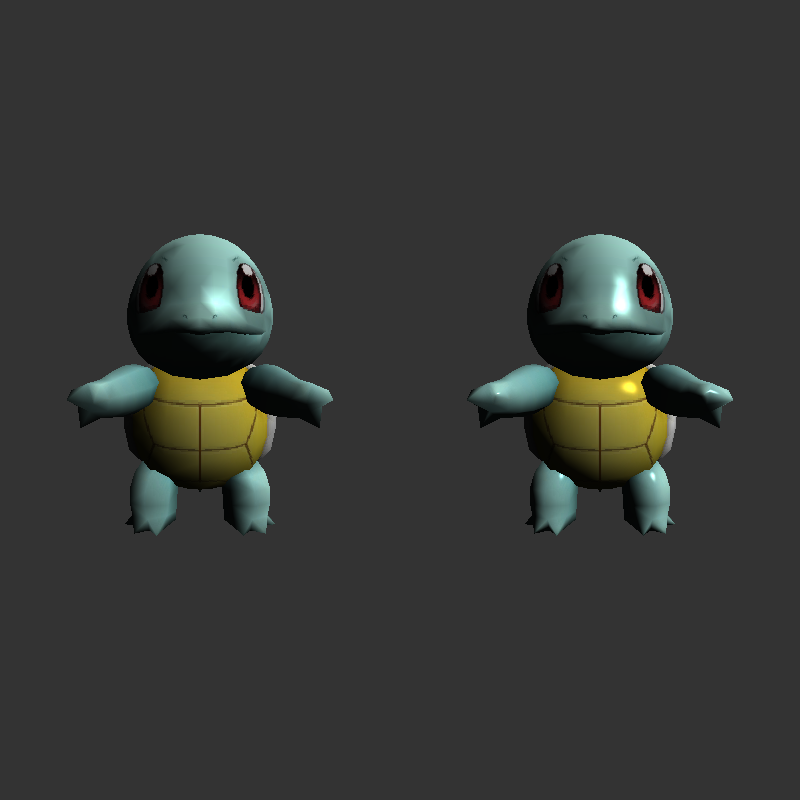
\includegraphics[width=0.5\textwidth]{type_b_model}
    \caption{Type B model}
  \end{figure}
\end{frame}

\begin{frame}
  \frametitle{Texture Filtering -- Magnification}
  \begin{figure}
    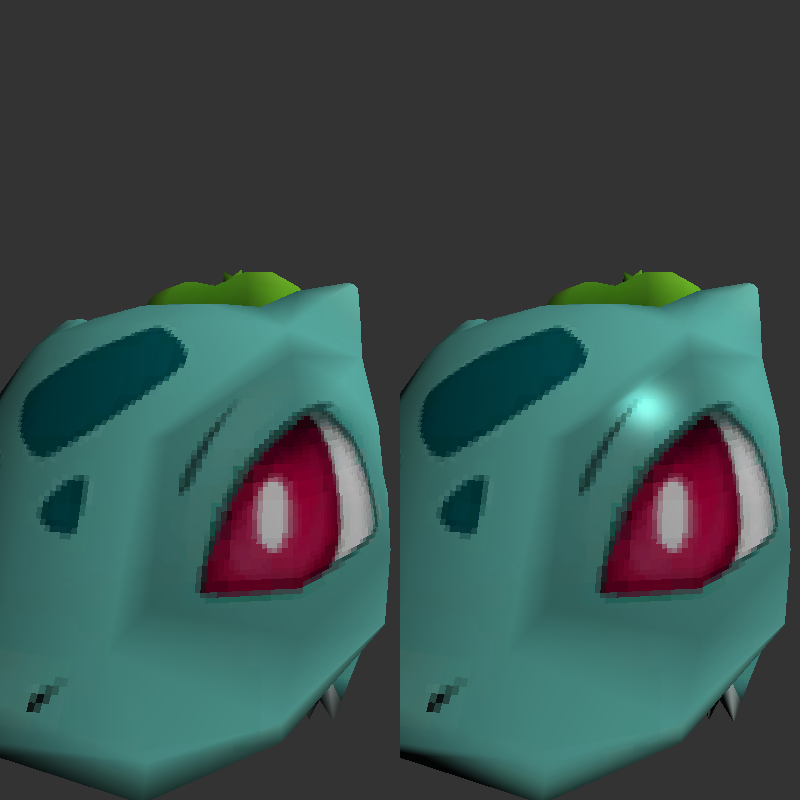
\includegraphics[width=0.5\textwidth]{nearest_magnification}
    \caption{Nearest magnification}
  \end{figure}
\end{frame}

\begin{frame}
  \frametitle{Texture Filtering -- Magnification (Continued)}
  \begin{figure}
    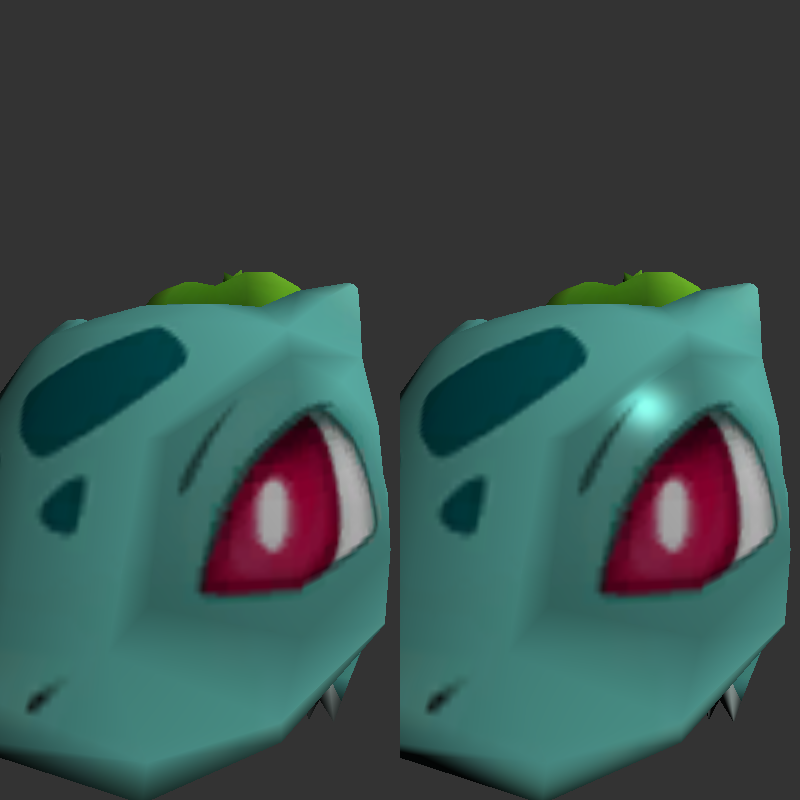
\includegraphics[width=0.5\textwidth]{linear_magnification}
    \caption{Linear magnification}
  \end{figure}
\end{frame}

\begin{frame}
  \frametitle{Texture Filtering -- Minification}
  \begin{figure}
    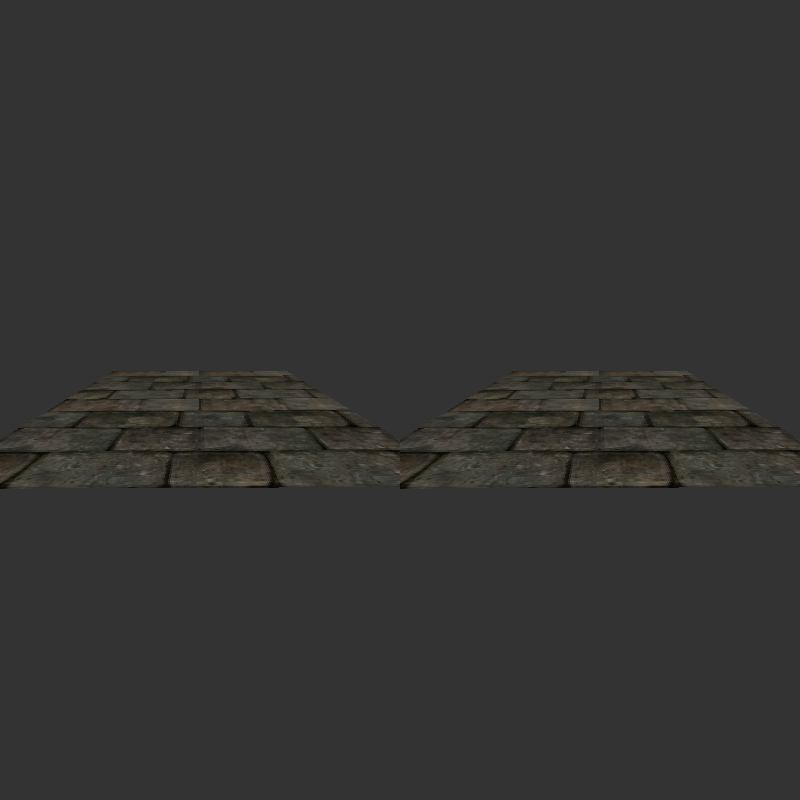
\includegraphics[width=0.5\textwidth]{nearest_minification}
    \caption{Nearest-mipmap-linear minification}
  \end{figure}
\end{frame}

\begin{frame}
  \frametitle{Texture Filtering -- Minification (Continued)}
  \begin{figure}
    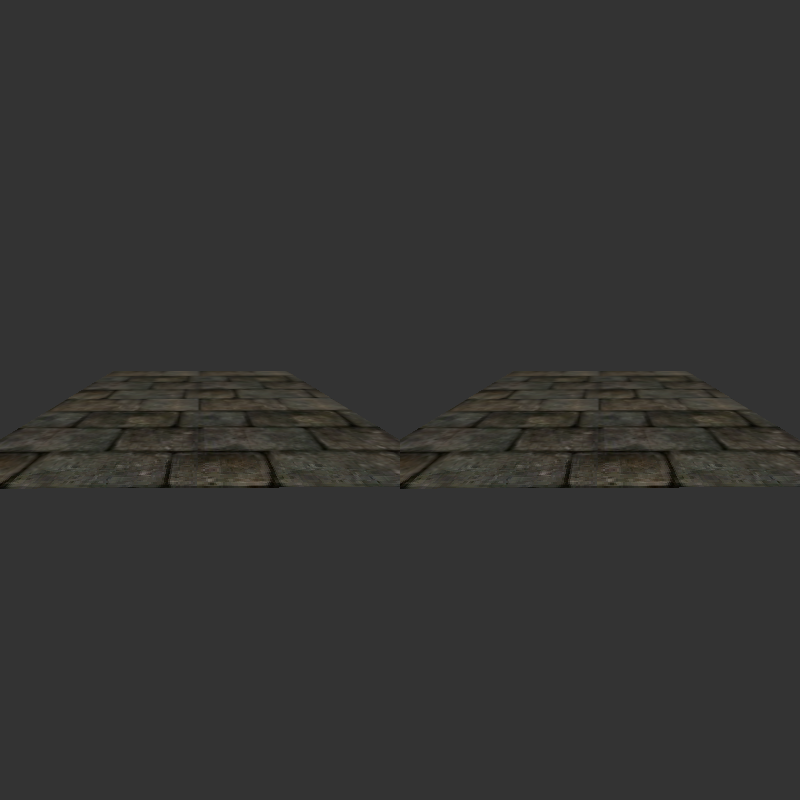
\includegraphics[width=0.5\textwidth]{linear_minification}
    \caption{Linear-mipmap-linear minification}
  \end{figure}
\end{frame}

\begin{frame}
  \frametitle{Texture Transform}
  \begin{figure}
    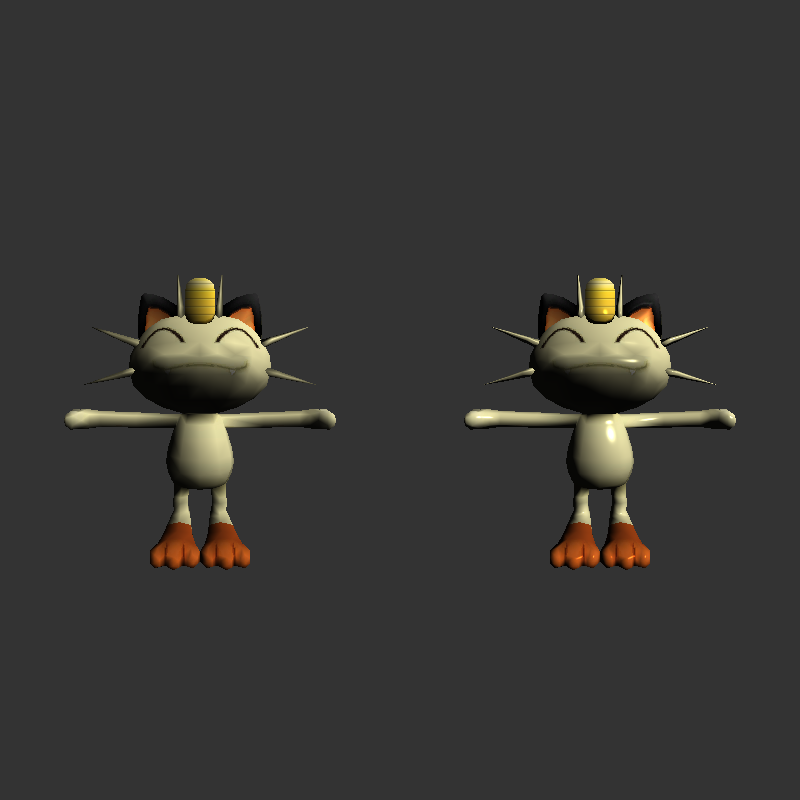
\includegraphics[width=0.5\textwidth]{eye_texture}
    \caption{Eye texture}
  \end{figure}
\end{frame}

\end{document}
